\documentclass[11pt]{exam}
\usepackage[utf8]{inputenc}
\usepackage[a4paper,top=2cm,left=2cm,right=2cm,bottom=2cm]{geometry}
\usepackage{import}
\usepackage[T1]{fontenc}
\usepackage[german,ngerman]{babel}
\usepackage[table]{xcolor}
\usepackage{amsthm, esvect}
\usepackage{mathtools}
\RequirePackage{amssymb, amsfonts, amsmath, latexsym, verbatim, xspace}
\usepackage{systeme}
\usepackage{multicol}
\usepackage{multirow}
\usepackage{framed}
\usepackage{array}
\usepackage{ragged2e}
\usepackage{graphicx}
\usepackage{pdflscape}
\usepackage{epstopdf}
\usepackage{booktabs}
\usepackage{pdfpages}
\usepackage{float} % Allows putting an [H] in \begin{figure} to specify the exact location of the figure
\usepackage{wrapfig} % Allows in-line images such as the example fish picture
\usepackage{tikz, graphicx} % tikz
\usepackage[position=top]{subfig}
\usepackage[bookmarks=true]{hyperref}%Links
\usepackage{enumerate}
\usepackage{enumitem}
\usepackage[german,ruled,vlined,linesnumbered,algosection]{algorithm2e}
\usepackage[labelfont=sf]{caption}
\usepackage{lmodern}
\usepackage{lscape}
\usepackage{tabularx}
\usepackage{systeme}
\usepackage{hhline}
\usepackage{subfiles}
\usepackage{stackengine}
\usepackage{setspace}
\usepackage{MnSymbol}
\usepackage{tcolorbox}
\usepackage{bbm}
\usepackage{url}
\usepackage{xparse}
\usepackage{sectsty}
\usepackage{array}
\usepackage{ragged2e}
\usepackage{listings} %Stellt Code-Snippets sauber dar

% definiert die Sprache
\selectlanguage{German}

% add command for different dates in Swiss fashion
\newcommand{\monthwordlong}[1]{\ifcase#1 \or Januar\or Februar\or März\or April\or Mai\or Juni\or Juli\or August\or September\or Oktober\or November\or Dezember\fi}
\newcommand{\monthwordshort}[1]{\ifcase#1\or Jan\or Feb\or Mar\or Apr\or Mai\or Jun\or Jul\or Aug\or Sept\or Okt\or Nov\or Dez\fi}
\newcommand{\datelong}{\number\day.\:\monthwordlong{\the\month}\:\number\year}
\newcommand{\dateshort}{\number\day.\:\monthwordshort{\the\month}\:\number\year}

% define color of links inside a text
\definecolor{linkblue}{RGB}{0, 0, 80}
\definecolor{plotblue}{RGB}{100, 100, 255}
\definecolor{myblue}{RGB}{8,164,214}
\definecolor{myred}{RGB}{143,42,41}
\definecolor{forestgreen}{RGB}{34,139,34}
\definecolor{highdive}{RGB}{10,169,194}
\definecolor{charcoal}{RGB}{74,74,74}
\hypersetup{
	colorlinks=true,
	linkcolor=linkblue,
	filecolor=magenta,
	urlcolor=plotblue,
	citecolor=linkblue,
	pdfpagemode=FullScreen,
}


\lstdefinestyle{mystyle}{ % definiert den style des Code-Snippets
	%backgroundcolor=\color{backcolour},
	%commentstyle=\color{codegreen},
	%keywordstyle=\color{magenta},
	%numberstyle=\tiny\color{codegray},
	%stringstyle=\color{codepurple},
	basicstyle=\ttfamily\footnotesize,
	breakatwhitespace=false,
	breaklines=true,
	captionpos=b,
	keepspaces=true,
	%numbers=left,
	%numbersep=5pt,
	showspaces=false,
	showstringspaces=false,
	showtabs=false,
	tabsize=4
}
\lstset{style=mystyle}
\qformat{\Large\textbf{Aufgabe \thequestion\hfill\thepoints}}
\newlist{partes}{enumerate}{3}
\setlist[partes]{label=(\alph*)}
\newcommand{\parte}{\item}
\newlist{subpartes}{enumerate}{3}
\setlist[subpartes]{label=\roman*)}
\newcommand{\subparte}{\item}
\setlist[enumerate,1]{%(
	leftmargin=*, itemsep=12pt, label={\textbf{\arabic*.)}}}
\newcommand\answerbox{%%
	\fbox{\rule{2in}{0pt}\rule[-0.1ex]{0pt}{4ex}}}
\pointpoints{Punkt}{Punkte}
\hqword{Frage:}
\hpword{Mögliche Punkte:}
\hsword{Erreicht:}
\htword{Total}
\renewcommand*\half{.5}
\renewcommand{\solutiontitle}{\noindent\textbf{Lösung:}\par\noindent}

% Graphed boxes
\newcommand{\karos}[2]{
  \begin{tikzpicture}
    \draw[step=0.4cm,color=cyan,dotted] (0,0) grid (#1 cm ,#2 cm);
  %  \draw((#1)/2 cm,0)--((#1)/2 cm,/#2)/2cm)
  \end{tikzpicture}
}
\usetikzlibrary{arrows, petri, topaths, graphs}
\linespread{1.2} % Line spacing

%=========================================================
\newenvironment{parcols}[1][]{
    \begin{parts}\begin{multicols}{#1}
}{
    \end{multicols}\end{parts}
}
%=========================================================
\newenvironment{itemcols}[1][]{
	\begin{itemize}\begin{multicols}{#1}
		}{
	\end{multicols}\end{itemize}
}

%=========================================================
\newcommand{\antwort}[1]{
	{\setlength{\textwidth}{\textwidth}\fillwithgrid{#1cm}\vspace{5pt}}
}

%=========================================================
% Karriertes Papier für Antwort MIT OVERLAY
\tcbuselibrary{breakable,skins}
\usetikzlibrary{mindmap,trees}
\newlength\tindent
\setlength{\tindent}{\parindent}
\setlength{\parindent}{0pt}
\setlength{\parskip}{0pt}

\newtcolorbox{gridspace}[1]{%
	enhanced,
	breakable,
	blanker,
	boxrule=0pt,
	left=5mm,
	right=5mm,
	top=5.75mm,
	bottom=0mm,
	boxsep=0pt,
	height=#1cm,
	width=16cm,
	before upper={
		\begingroup
		\setlength{\baselineskip}{5.75mm}
		\setlength{\parskip}{0pt}
		\setlength{\lineskip}{0pt}
		% keep every paragraph on the grid rhythm
		%\everypar{\vspace{0pt}\strut}
		% math formulas shifted by one grid row
		\let\oldbracketopen\[
		\renewcommand{\[}{\vspace{-5mm}\oldbracketopen}
		% Align displayed formulas to the grid
		\setlength{\abovedisplayskip}{0pt}
		\setlength{\belowdisplayskip}{0pt}
		\setlength{\abovedisplayshortskip}{0pt}
		\setlength{\belowdisplayshortskip}{0pt}
		% Enumerate follows the same rhythm
		\setlist[enumerate]{leftmargin=6mm,itemsep=0mm,topsep=0pt,parsep=0pt,partopsep=0pt}
		\setlist[itemize]{leftmargin=6mm,itemsep=10mm,topsep=0pt,parsep=0pt,partopsep=0pt}},
	after upper={
		\endgroup},
	underlay={
		\draw[step=5mm,color=gray!55] (interior.south west) grid (interior.north east);}
}

\pagestyle{headandfoot}
\firstpageheader{}{}{\teacher}
\runningheader{}{}{\teacher}
\firstpagefooter{}{}{Seite \thepage\:von \numpages}
\runningfooter{}{}{Seite \thepage\:von \numpages}
%%
% Math Arrows
%%
\newcommand{\same}{\ensuremath{\Longleftrightarrow}}
\renewcommand{\to}{\ensuremath{\longrightarrow}}
\newcommand{\qsame}{\quad\same\quad}
\newcommand{\dsame}{\ensuremath{:\Leftrightarrow}}
\newcommand{\qdsame}{\quad\dsame\quad}
\newcommand{\ldsame}{\ensuremath{:\Longleftrightarrow}}
\newcommand{\samedef}{\ensuremath{\us {\text{def}} \Leftrightarrow}}
\newcommand{\qsamedef}{\quad\samedef\quad}
\newcommand{\lsamedef}{\ensuremath{\us {\text{def}} \Longleftrightarrow}}
\newcommand{\qlsamedef}{\quad\lsamedef\quad}


%%
% Mengendefinitionen
%%
\newcommand{\M}{\ensuremath{\mathcal{M}}}
\newcommand{\N}{\ensuremath{\mathbb{N}}}
\newcommand{\Z}{\ensuremath{\mathbb{Z}}}
\newcommand{\Q}{\ensuremath{\mathbb{Q}}}
\newcommand{\I}{\ensuremath{\mathbb{I}}}
\newcommand{\R}{\ensuremath{\mathbb{R}}}
\newcommand{\C}{\ensuremath{\mathbb{C}}}
\renewcommand{\S}{\ensuremath{\mathbb{S}}}
\newcommand{\Prim}{\ensuremath{\mathbb{P}}}
\newcommand{\0}{\ensuremath{\emptyset}}
\renewcommand{\Re}{\ensuremath{\operatorname{Re}}}
\renewcommand{\Im}{\ensuremath{\operatorname{Im}}}
\newcommand{\strich}{\ensuremath{\big\vert}}

%%
% Mengenoperation
%%
\renewcommand{\nin}{\not\in}


%%
% Logisches Und und Oder
%%
\newcommand{\sand}{\ensuremath{\; \land \;}}
\newcommand{\sor}{\ensuremath{\; \lor \;}}
\renewcommand{\*}{\ensuremath{\cdot}}
\newcommand{\oder}{\vee}
\newcommand{\n}{\neg}
\newcommand{\und}{\wedge}


%%
% Bei Integral, Summe,... die Grenzen über bzw.
% unter das Zeichen
%%
\renewcommand{\d}[1]{\ensuremath{\operatorname{d}\!{#1}}}
\newcommand{\Sum}{\sum\limits}
\newcommand{\Prod}{\prod\limits}
\newcommand{\Min}{\min\limits}
\newcommand{\Max}{\max\limits}
\newcommand{\Lim}{\lim\limits}
\newcommand{\Inf}{\inf\limits}
\newcommand{\Sup}{\sup\limits}
\newcommand{\Liminf}{\liminf\limits}
\newcommand{\Limsup}{\limsup\limits}
%\renewcommand{\Cup}{\bigcup\limits}
%\renewcommand{\Cap}{\bigcap\limits}
\newcommand{\Otimes}{\bigotimes\limits}
\newcommand{\Oplus}{\bigoplus\limits}


%%
% Arcus Cotangens, Logarithmus
%%
\let\oldsin\sin
\renewcommand{\sin}[1]{\oldsin{\left(#1\right)}}
\let\oldcos\cos
\renewcommand{\cos}[1]{\oldcos{\left(#1\right)}}
\let\oldtan\tan
\renewcommand{\tan}[1]{\oldtan{\left(#1\right)}}
\let\oldarcsin\arcsin
\renewcommand{\arcsin}[1]{\oldarcsin{\left(#1\right)}}
\let\oldarccos\arccos
\renewcommand{\arccos}[1]{\oldarccos{\left(#1\right)}}
\let\oldarctan\arctan
\renewcommand{\arctan}[1]{\oldarctan{\left(#1\right)}}
\let\oldln\ln
\renewcommand{\ln}[1]{\oldln{\left(#1\right)}}
\newcommand{\Log}[2]{\ensuremath{\operatorname{log}_{#1}\left(#2\right)}}
\newcommand{\e}{\operatorname{e}}
\renewcommand{\exp}[1]{\ensuremath{\operatorname{\e}^{#1}}}


%%
% Griechische Buchstaben
%%
\renewcommand{\epsilon}{\ensuremath{\varepsilon}}
\renewcommand{\phi}{\varphi}
\renewcommand{\l}{\lambda}
\renewcommand{\t}{\tau}


%%
% Bezeichnungen
%%
\newcommand{\Rgn}{\R_{>0}} % R grösser Null
\newcommand{\Rad}{\operatorname{Rad}}   % Radikal
\newcommand{\kgV}{\operatorname{kgV}}   % Kleinster gemeinsame Vielfache
\newcommand{\ggT}{\operatorname{ggT}}   % Grösster gemeinsame Teiler
\newcommand{\winkel}{\sphericalangle}          % Winkelsymbol
\DeclarePairedDelimiter\abs{\lvert}{\rvert} % besserer Betrag
\makeatletter
\let\oldabs\abs
\def\abs{\@ifstar{\oldabs}{\oldabs*}}
\makeatother


%%
% Vektorgeometrie
%%
\renewcommand{\v}[1]{\vv{#1}}       % besserer Pfeil über Buchstaben
\renewcommand{\vec}[2]{\begingroup\renewcommand{\arraystretch}{1}\left(\begin{array}{c} #1 \\ #2 \end{array}\right)\endgroup}   % two dimensional vector
\renewcommand{\Vec}[3]{\begingroup\renewcommand{\arraystretch}{1}\left(\begin{array}{c} #1 \\ #2 \\ #3 \end{array}\right)\endgroup}      % three dimensional vector


%%
% Text
%%
\newcommand*{\Ueq}[1]{\mathrel{\mathop{=}\limits_{\text{#1}}}}
\newcommand*{\Oeq}[1]{\mathrel{\stackrel{\text{#1}}{=}}}
\newcommand{\utext}[2]{\underbrace{#1}_{\substack{#2}}}
\newcommand{\otext}[2]{$\overbrace{\textrm{#1}}^{\textrm{#2}}$}
\newcommand{\lineortext}[1]{\hspace{0,1cm}\underline{\hspace{0.1cm}\hphantom{#1}\hspace{0.1cm}}\hspace{0,1cm}} % Lückentext erstellen
\newcommand{\gap}[1]{\rule{#1 cm}{1pt}}
%=========================================================
\newcommand{\theme}{Einführung Funktion}
\newcommand{\teacher}{Jonas Guler}
%=========================================================
\begin{document}
\fontsize{14}{14}\selectfont
\begin{center}
    \huge\bf\theme
\end{center}

\begin{questions}
%=========================================================
%-------------------TESTFRAGEN
%=========================================================
\question[4] %DMKA910 - Anhang2 A1
Begründe für die folgenden Abbildungen, ob es sich dabei um eine Funktion handelt.
\begin{parts}
    \part
    \begin{minipage}{0.2\linewidth}
        \centering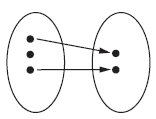
\includegraphics[scale=1]{data-algebra/Fkt1.png}
    \end{minipage}
    \hfill
    \begin{minipage}{0.7\linewidth}
        \antwort{6}
    \end{minipage}
    \vspace{1cm}\part
    \begin{minipage}{0.2\linewidth}
        \centering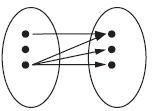
\includegraphics[scale=1]{data-algebra/Fkt2.png}
    \end{minipage}
    \hfill
    \begin{minipage}{0.7\linewidth}
        \antwort{6}
    \end{minipage}
    \vspace{1cm}\part
    \begin{minipage}{0.2\linewidth}
        \centering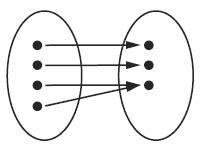
\includegraphics[scale=0.75]{data-algebra/Fkt3.png}
    \end{minipage}
    \hfill
    \begin{minipage}{0.7\linewidth}
        \antwort{6}
    \end{minipage}
    \vspace{1cm}\part
    \begin{minipage}{0.2\linewidth}
        \centering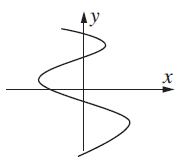
\includegraphics[scale=1]{data-algebra/Fkt4.png}
    \end{minipage}
    \hfill
    \begin{minipage}{0.7\linewidth}
        \antwort{6}
    \end{minipage}
    \vspace{1cm}\part
    \begin{minipage}{0.2\linewidth}
        \centering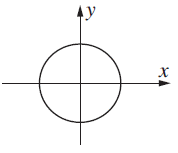
\includegraphics[scale=1]{data-algebra/Fkt5.png}
    \end{minipage}
    \hfill
    \begin{minipage}{0.7\linewidth}
        \antwort{6}
    \end{minipage}
\end{parts}

%---------------------------------------------------------
\question[7] %
Eine Funktion $f$ ist gebend durch seine Funktionsgleichung
\[f:y=\frac{x+2}{x}.\]
\begin{parts}
    \part Gib den grösst möglichen Definitionsbereich $D_f$ an.
    \part Gib den Wertebereich $W_f$ an.
    \part Berechne die folgenden Funktionswerte: $f(3),\quad f(-2), \quad\text{ und } f(m)$.
    \part Liegen die folgenden Punkte auf dem Graph der Funktion $f$?
    \[P=\left(4,\frac{3}{2}\right), \quad Q=\left(-2,-1\right),\quad\text{ und } R=\left(t-1,\frac{t+1}{t-1}\right)\]
\end{parts}

%---------------------------------------------------------
\question[7] %DMK A910 - Anhang2 A9
Eine Funktion $f$ ist geben durch seine Funktionsgleichung
\[f:y=\frac{x-1}{x}.\]
\begin{parts}
    \part Gib den grösst möglichen Definitionsbereich $D_f$ an.
    \part Gib den Wertebereich $W_f$ an.
    \part Berechne die folgenden Funktionswerte: $f(2),\quad f(-1), \quad\text{ und } f(m)$.
    \part Liegen die folgenden Punkte auf dem Graph der Funktion $f$?
    \[P=(1,0), \quad Q=\left(\frac{1}{3},-2\right),\quad\text{ und } R=\left(t-1,\frac{t-2}{t-1}\right)\]
\end{parts}

%---------------------------------------------------------
\question[8] %
Eine Funktion $f$ ist gebend durch seine Funktionsgleichung
\[f:y\mapsto\frac{3x}{2x-1}.\]
\begin{parts}
    \part Gib den grösst möglichen Definitionsbereich $D_f$ und den Wertebereich $W_f$ an.
    \part Berechne die folgenden Funktionswerte: $f(3),\quad f(-2), \quad\text{ und } f(m-2)$.
    \part Berechne das jeweilige Argument $x$, wenn $f(x)=\frac{1}{2}$.
    \part Liegen die folgenden Punkte auf dem Graph der Funktion $f$?
    \[P=\left(1,3\right), \quad Q=\left(\frac{1}{3},-1\right),\quad\text{ und } R=\left(t-1,\frac{3t-3}{2t-1}\right)\]
\end{parts}

%---------------------------------------------------------
\question[4] %DMKA910 - Anhang2 A11
\begin{minipage}{0.45\linewidth}
    Gegeben ist der Graph einer Funktion $f$. Antworte anhand der nebenstehenden Darstellung.
    \begin{parts}
        \part Für welche Argumente $x$ ist $f(x)=3$?
        \part Welchen Wert hat $f(0)$ und $f(2)$?
    \end{parts}
\end{minipage}
\hfill
\begin{minipage}{0.45\linewidth}
    \centering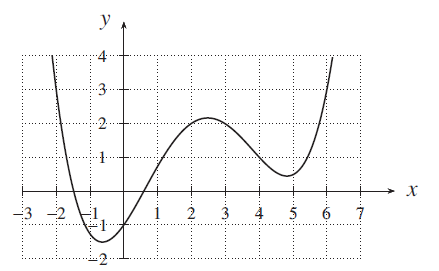
\includegraphics[scale=0.65]{data-algebra/GraphGaMa.png}
\end{minipage}

%---------------------------------------------------------
\question[6] %DMKA910 - S59 A21
Sind die folgenden Aussagen richtig oder falsch? Begründe deine Antwort.
\begin{parts}
    \part Der Abstand von zwei parallelen Geraden ist der Unterschied der beiden y-Achsenabschnitte.
    \part Die Steigung $m=-\frac{9}{27}$ gehört zu einer Gerade, die auf drei Einheiten in x-Richtung eine Einheit in y-Richtung fällt.
    \part Jede Gerade durch zwei Punkte ist der Graph einer linearen Funktion.
\end{parts}

%---------------------------------------------------------
\noaddpoints
\question[\totalpoints] % Funktionsgleichung und Graph
\addpoints
Betrachte die beiden Punkte $A=(-6,-8)$ und $B=(5,9)$.
\begin{parts}
    \part[2] Zeichne die Funktion $f$ ins Koordinatengitter rechts ein.
    \part[4] Gib die Funktionsgleichung der linearen Funktion $f$ an.
\end{parts}

\begin{figure}[H]
    \begin{tikzpicture}[cross/.style={draw, cross out, minimum size=2*(#1-1pt), inner sep=0pt, outer sep=0pt}, x=5mm, y=5mm,
        >=latex,   %Voreinstellung für Pfeilspitzen
        font=\footnotesize, scale=0.8]
        %Raster zeichnen
        \draw [color=gray!50]  [step=5mm] (-7.3,-9.3) grid (7.3,10.3);
        % Achsen zeichnen
        \draw[->,thick] (-7.3,0) -- (7.8,0) node[left, below] {\normalsize $x$};
        \draw[->,thick] (0,-9.3) -- (0,10.8) node[above, left=4pt] {\normalsize $y$};
        % Achsen beschriften
        \foreach \x in {-6,-4,-2,2,4,6} \draw (\x,-.1) -- (\x,.1) node[below=4pt] {$\x$};
        \foreach \y in {-8,-6,-4,-2,2,4,6,8,10} \draw (-.1,\y) -- (.1,\y) node[left=4pt] {$\y$};
        % Besserer Ursprung
        \draw[color=black] (0pt,-7pt) node[left] {$0$};
        %Funktionen zeichnen:
        \clip(-7.3,-9.3) rectangle (7.3,10.3); %Bildbereich
        %Beschriftung
        %\node[forestgreen]  at (3.2,1) {\normalsize$g$};
    \end{tikzpicture}
\end{figure}

%---------------------------------------------------------
\noaddpoints
\question[\totalpoints] %Funktiongleichung finden
\addpoints
Betrachte die beiden Punkte $A=(-9,4)$ und $B=(6,-5)$.
\begin{parts}
    \part[2] Gib die Funktionsgleichung der linearen Funktion $f$ an.
    \part[4] Zeichne die Funktion $f$ ins Koordinatengitter rechts ein.
\end{parts}
\begin{figure}[H]
    \begin{tikzpicture}[cross/.style={draw, cross out, minimum size=2*(#1-1pt), inner sep=0pt, outer sep=0pt}, x=5mm, y=5mm,
        >=latex,   %Voreinstellung für Pfeilspitzen
        font=\footnotesize, scale=0.8]
        %Raster zeichnen
        \draw [color=gray!50]  [step=5mm] (-7.3,-9.3) grid (7.3,10.3);
        % Achsen zeichnen
        \draw[->,thick] (-7.3,0) -- (7.8,0) node[left, below] {\normalsize $x$};
        \draw[->,thick] (0,-9.3) -- (0,10.8) node[above, left=4pt] {\normalsize $y$};
        % Achsen beschriften
        \foreach \x in {-6,-4,-2,2,4,6} \draw (\x,-.1) -- (\x,.1) node[below=4pt] {$\x$};
        \foreach \y in {-8,-6,-4,-2,2,4,6,8,10} \draw (-.1,\y) -- (.1,\y) node[left=4pt] {$\y$};
        % Besserer Ursprung
        \draw[color=black] (0pt,-7pt) node[left] {$0$};
        %Funktionen zeichnen:
        \clip(-7.3,-9.3) rectangle (7.3,10.3); %Bildbereich
        %Beschriftung
        %\node[forestgreen]  at (3.2,1) {\normalsize$g$};
    \end{tikzpicture}
\end{figure}

%---------------------------------------------------------
\noaddpoints
\question[\totalpoints]
\addpoints
Aus einem tropfenden Wasserhahn fällt alle $1.5$ Sekunden ein Tropfen in einen Messbecher. Momentan (zur Zeit $t=0$) sind darin $90$ ml enthalten.\newline ($20$ Tropfen $\widehat{=}\:1$ ml)
\begin{parts}
    \part[2] Fülle die Lücken dieser Wertetabelle aus.
    \begingroup
    \renewcommand{\arraystretch}{1.5}
    \begin{table}[H]
        \centering
        \begin{tabular}{|c|p{12mm}|p{12mm}|p{12mm}|p{12mm}|p{12mm}|}\hline
            Vergangene Zeit $t$ in Minuten & $0$ &  &  & $4$ & $80$ \\\hline
            Wassermenge $f(t)$ im Becher in ml & $90$ & $180$ & $330$ & & \\\hline
        \end{tabular}
    \end{table}
    \endgroup
    \part[3] Gib die Funktionsgleichung an, mit der die Wassermenge aus der Zeit berechnet werden kann.
    \part[2] Wie lange dauert es, bis einen Liter Wasser im Messbecher ist?
\end{parts}

%---------------------------------------------------------
\noaddpoints
\question[\totalpoints]
\addpoints
Betrachte die beiden linearen Funktionen $f(x)=\frac{2}{3}x-3$ und $g(x)=\frac{4}{5}x+1$.
\begin{parts}
    \part[4] Berechne die Koordinaten des Schnittpunktes der Funktionen $f$ und $g$. % Algebra 9/10 S58 A17b)
    \part[2] Erkläre in deinen Worten, warum die Koordinaten des Schnittpunktes als Lösung eines linearen Gleichungssystems aufgefasst werden kann. Gib das zugehörige Gleichungssystem an.
\end{parts}

%---------------------------------------------------------
\question[9] %Anwendung mit Schnittpunkt DMKA910 - S58 A20
In einer Mathematikprüfung mit total $24$ Punkten ergeben $0$ Punkte die Note $1$ und $20$ Punkte die Note $6$. Es gibt nur ganze und halbe Punkte. Die Notenskala ist linear.
\begin{parts}
    \part Gib die Gleichung der Funktion an die jeder Punktzahl $P$ eine Note $N$ zuordnet.
    \part Welche Note erhält Mia für $15$ erreichte Punkte?
    \part Welche Punktzahl benötigt Leon mindestens, um eine Note $4$ zu erreichen?
    \part Am gleichen Tag schrieb die Klasse ein Deutschdiktat. Dabei wird pro zwei Fehler eine halbe Note abgezogen. Mit zwei Fehlern bekommt man immer noch die Note $6$. Wie viele Fehler dürfen im Diktat gemacht werden bzw. wie viele Punkte müssen in der Mathematikprüfung erreicht werden, um in beiden Prüfungen die exakt gleiche Note zu erhalten?
\end{parts}

%---------------------------------------------------------
\question[9] %Anwendung mit Schnittpunkt
Ein Fallschirmspringer hat $20$ Sekunden nach dem Öffnen des Fallschirms noch eine Höhe von 250 Meter über Boden. Er sinkt in jeder Sekunde um 5 Meter.
\begin{parts}
    \part Stelle eine Funktionsgleichung auf, die die verstichene Zeit (in Sekunden) der Höhe über Boden zuordnet.
    \part In welcher Höhe wurde der Fallschirm geöffnet?
    \part Wie lange dauert es, von der Öffnung des Fallschirms bis der Springer wieder am Boden ist?
    \part Direkt neben dem Landeplatz des Springers startet gleichzeitig mit dem Öffnen des Fallschirms ein Flugzeug, um weitere Springer in die Luft zu bringen. Nach $1$ Minute ist das Flugzeug bereits $540$ Meter über dem Boden. Zu welcher Zeit ist das Flugzeug gleich hoch wie der fallende Fallschirmspringer?
\end{parts}


%---------------------------------------------------------
\question[2]
Entscheide in der Tabelle unten, ob die Aussagen wahr oder falsch sind. Die Antworten müssen nicht begründet werden.\newline
\begin{small}
    Bewertung: Für $0-2$ korrekte Antworten gibt es keine Punkte; $3$ korrekte Antworten einen Punkt und falls alle Antworten korrekt sind, gibt es $2$ Punkte.
\end{small}
\begingroup
\renewcommand{\arraystretch}{1.5}
\begin{table}[h]
    \centering
    \begin{tabular}{|p{12cm}|c|c|}\hline
         & wahr & falsch \\\hline
        Jede Gerade durch zwei Punkte ist der Graph einer linearen Funktion. & & \\\hline
        In einer Funktion darf jedes Bild maximal ein Argument haben. & & \\\hline
        Das Produkt der Steigungen zweier senkrecht aufeinander stehender Geraden ist stets $-1$. & & \\\hline
        Alle linearen Gleichungssysteme haben mindestens eine Lösung. & & \\\hline
    \end{tabular}
\end{table}
\endgroup






\end{questions}
\end{document}